
\newpage
\chapter{Stromstärke- und Spannungsmessung}

Zwei der grundlegenden Grössen in der Elektriztitätslehre sind die Spannung $U$ und die Stromstärke $I$.
Ein elektrischer Strom entsteht, wenn sich elektrische Ladungen bewegen.
Die Spannung ist die Ursache dafür, dass diese sich bewegen. Ist die Spannung null, fliesst kein elektrischer Strom.

Im Wassermodell sieht
man das sehr gut, siehe \fref{fig:watermodel}. Ist der Höhenunterschied zwischen den Tanks null, fliesst kein
Wasser durch die Rohre.

Gibt es eine Spannung und ist der Stromkreis geschlossen, fliesst ein elektrischer Strom.
Die Stromstärke ist die Menge an Ladung, die durch einen bestimmten Zeitraum fliesst.
Im Wassermodell entspricht die Stromstärke der Flussrate des Wassers, d.h. wie viel Wasser pro Sekunde
an einer Stelle im Rohr durchfliesst.


\section{Stromstärkemessung}

Die Stromstärke $I$ ist definiert als das Verhältnis zwischen der Ladung $Q$ und der Zeit $t$,
die benötigt wird, um diese Ladung zu transportieren. Die Einheit der Stromstärke ist
Ampere ($\unit{\ampere}$).

\begin{greenbox}
\textbf{Stromstärke $I$}
$$
    I = \frac{Q}{t} \quad,\quad \left[ I \, \right] = \frac{\unit{\coulomb}}{\unit{\second}} = \unit{\ampere} \quad \text{(Ampere)}
$$
\end{greenbox}


Betrachten wir nun die Messung der elektrischen Stromstärke $I$. Man verwendet dazu ein
Stromstärkemessgerät, auch Amperemeter genannt.

\begin{figure}[h!]
    \centering
    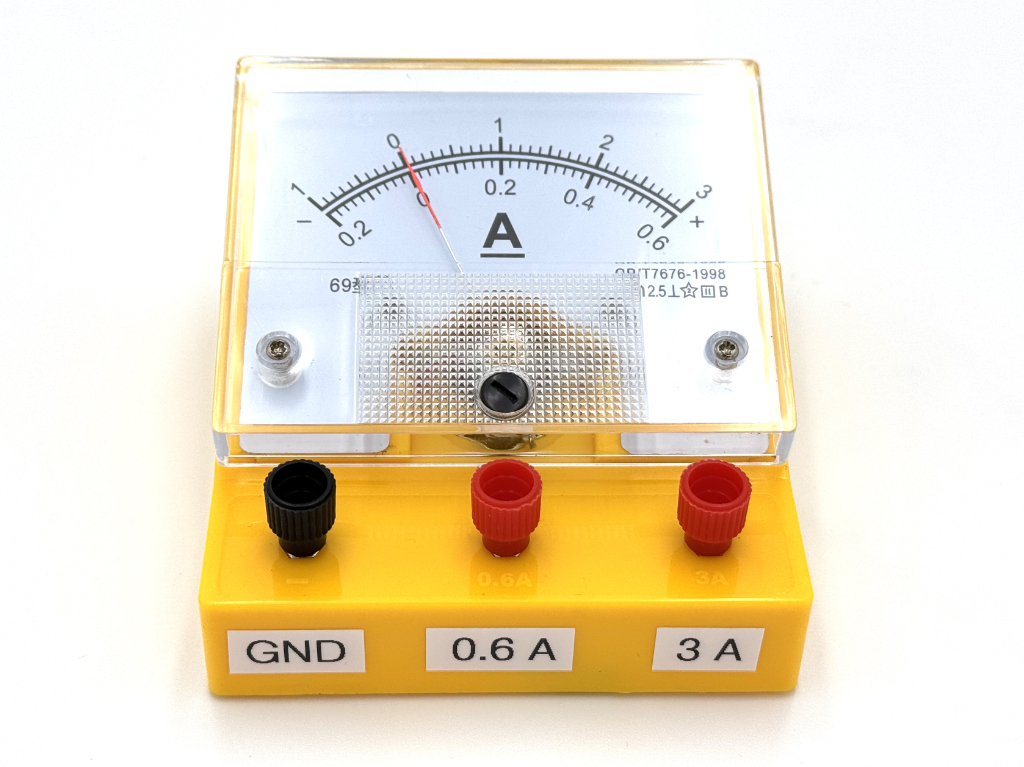
\includegraphics[width=6cm]{_images/ampere_meter}
    \caption{Stromstärkemessgerät, auch Amperemeter genannt.}
    \label{fig:amperemeter}
\end{figure}

Das Messgerät besteht aus einem Zeiger mit einer Skala, die die Stromstärke in Ampere darstellt.
Es hat drei Anschlüsse (GND), (0.6 A) und (3 A). Dies sind die beiden Messbereiche des Amperemeters.
Betrachtet man die Skala genau, sieht man, dass sie zweigeteilt ist. Die obere Skala zeigt
den Messbereich von -1 bis 3 Ampere, während die untere Skala den Bereich von -0.2 bis 0.6 Ampere abdeckt.


\newpage
\experiment{Stromstärkemessung}


Baue das Experiment aus siehe \fref{fig:current_measurement} auf.

\begin{figure}[h!]
    \centering
    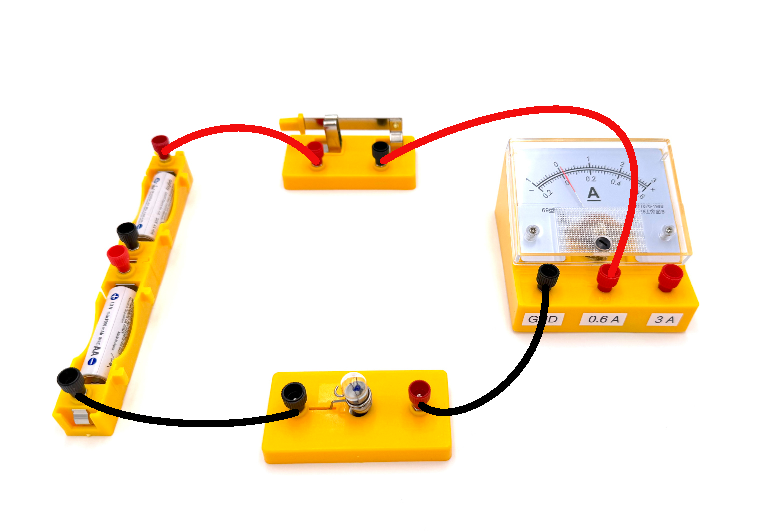
\includegraphics[width=9cm]{_images/ampere_setup.pdf}
    \caption{Stromstärkemessung}
    \label{fig:current_measurement}
\end{figure}

Schliesse den Schalter und notiere deine Beobachtungen. Beantworte die folgenden Fragen:

\begin{enumerate}
    \item Miss die Stromstärke mit dem Amperemeter (0.6 A).
    \item Miss die Stromstärke mit dem Amperemeter (3 A).
    \item Vertausche die beiden Kabel beim Amperemeter.
    \item Vervollständige den Schaltplan.
\end{enumerate}


% Raster für die Antworten
\begin{tikzpicture}
    \draw[step=4mm,gray,very thin] (0,0) grid (14.8,-8.4);

    \noanswer{
        \node  at (7,-6)
            {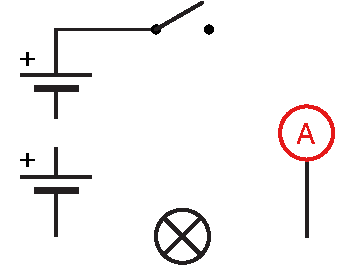
\includegraphics[width=6cm]{_images/ampere_setup_schaltplan.pdf}};
    }

    \answer{
        \node  at (7,-6)
            {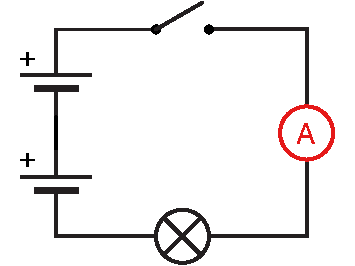
\includegraphics[width=6cm]{_images/ampere_setup_schaltplan_loesung.pdf}};
    }

    \answer{
        \draw (0.3,0.14) node[anchor=north west,align=left,text width=13cm] {%
      		\marker%

            \textbf{1.} Es fliessen ca. 0.26 A. \\
            \textbf{2.} Der Ausschlag der Nadel ist beim 3 A-Bereich kleiner Es fliesen etwas mehr als 0.2 A.\\
            \textbf{3.} Die Nadel schlägt in die negative Richtung aus.\\

        };
    }
\end{tikzpicture}


\newpage

\section{Kurzschluss bei der Stromstärkemessung}

Bei der Strommessung besteht die Gefahr, dass man das Amperemeter falsch anschliesst.
Es kann dann zu einem Kurzschluss kommen, welches in der Regel die Sicherung des
Amperemeters durchbrennen lässt, siehe \ref{fig:amperemeter_short_circuit}.

\begin{figure}[h!]
    \centering
    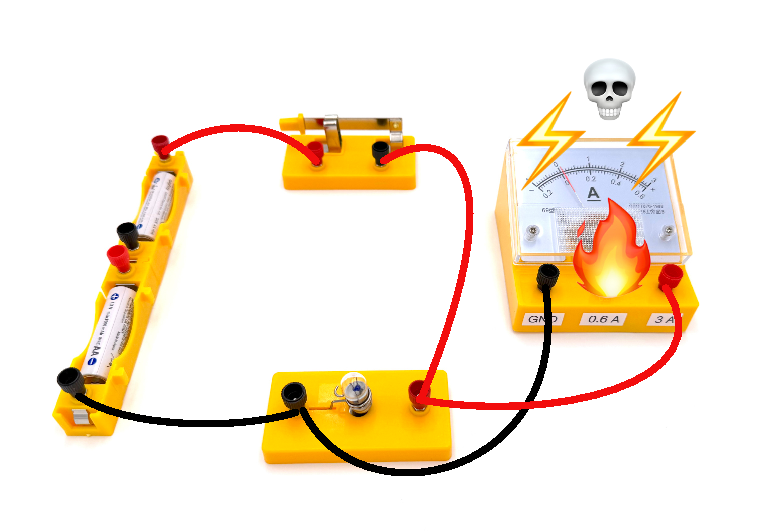
\includegraphics[width=8cm]{_images/ampere_kurzschluss}
    \caption{Kurzschluss mit dem Amperemeter}
    \label{fig:amperemeter_short_circuit}
\end{figure}

\begin{redbox}
Das Amperemeter darf nie parallel zum Verbraucher oder zur Batterie angeschlossen werden.
Es muss immer seriell, d.h. vor oder nach einem Verbraucher eingefügt werden.
\end{redbox}

Das Amperemeter hat die Aufgabe, den Stromfluss zu messen. Dafür muss es den elektrischen Strom
möglichst gut leiten. Man kann sich das Amperemeter wie ein Stück einer Leitung vorstellen.
Schaltet man das Amperemeter parallel zur Batterie, fliesst ein sehr grosser Strom
durch das Amperemeter und es entsteht ein Kurzschluss.


\exercise{Korrekte Stromstärkemessung}

Gib bei den folgenden Schaltplänen an, wo das Amperemeter richtig und wo falsch angeschlossen ist.

% Raster für die Antworten
\begin{tikzpicture}
    \draw[step=4mm,gray,very thin] (0,0) grid (14.8,-6);

    \node at (1,-0.6) {a)};
    \node  at (3.5,-3)
        {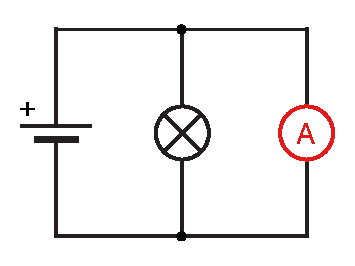
\includegraphics[width=6cm]{_images/ampere_kurzschluss_1.pdf}};

    \node at (8,-0.6) {b)};
    \node  at (10.5,-3)
        {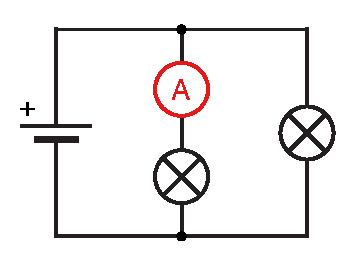
\includegraphics[width=6cm]{_images/ampere_kurzschluss_2.pdf}};

    \answer{
        \draw (1.4,-0.2) node[anchor=north west,align=left,text width=13cm] {%
      		\marker%
            falsch !! Achtung!
        };
        \draw (1.4,-5) node[anchor=north west,align=left,text width=13cm] {%
      		\marker%
        parallel zur Batterie!!!
        };


        \draw (8.4,-0.2) node[anchor=north west,align=left,text width=13cm] {%
      		\marker%
            korrekt
        };
        \draw (8.4,-5) node[anchor=north west,align=left,text width=13cm] {%
      		\marker%
            In Serie zum Verbraucher.
        };
    }
\end{tikzpicture}


\newpage
\experiment{Stromstärke in der Serienschaltung}

In diesem Experiment soll untersucht werden, wie gross die Stromstärke in einer Serienschaltung ist.
Das Amperemeter wird dazu nacheinander an verschiedenen Stellen im Stromkreis platziert.

\begin{figure}[h!]
\centering
    \begin{subfigure}[b]{0.305\textwidth}
    \centering
    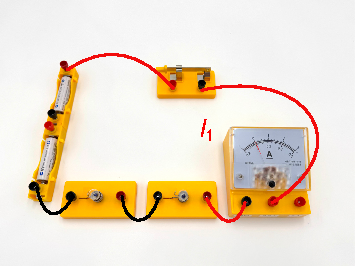
\includegraphics[width=4.6cm]{_images/ampere_serie_1.pdf}
    \end{subfigure}
\quad
    \begin{subfigure}[b]{0.305\textwidth}
    \centering
    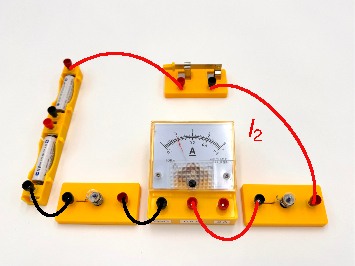
\includegraphics[width=4.6cm]{_images/ampere_serie_2.pdf}
    \end{subfigure}
\quad
    \begin{subfigure}[b]{0.305\textwidth}
    \centering
    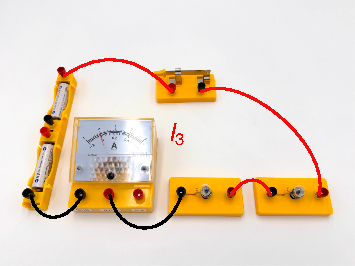
\includegraphics[width=4.6cm]{_images/ampere_serie_3.pdf}
    \end{subfigure}
\end{figure}


% Raster für die Antworten
\begin{tikzpicture}
    \draw[step=4mm,gray,very thin] (0,0) grid (14.8,-16);

    \node  at (3.5,-3.5)
        {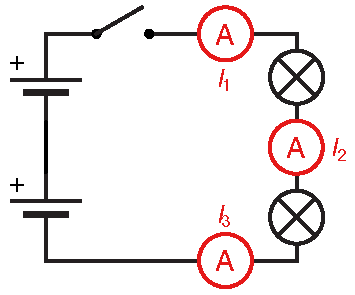
\includegraphics[width=6cm]{_images/ampere_serie}};

        \draw (8,-1.85) node[anchor=north west,align=left,text width=13cm] {%
      		\marker%

            I$_{\text{1}}$ = \answer{0.8 A}  \\
            I$_{\text{2}}$ = \answer{0.8 A} \\
            I$_{\text{3}}$ = \answer{0.8 A}  \\

        };

        \draw (1,-6.6) node[anchor=north west,align=left,text width=13cm] {%
      		\marker%

            Fazit\\
            \answer{Die Stromstärke in einer Serienschaltung ist überall\\
             gleich gross.}

        };
\end{tikzpicture}


\newpage
\experiment{Stromstärke in der Parallelschaltung}

In diesem Experiment werden die Stromstärken in einer Parallelschaltung untersucht.
Es wird die Gesamtstromstärke der beiden Lampen gemessen. Anschliessend wird das
Amperemeter nacheinander vor den einzelnen Lampen eingebaut.

\begin{figure}[h!]
\centering
    \begin{subfigure}[b]{0.305\textwidth}
    \centering
    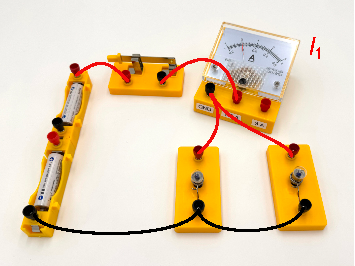
\includegraphics[width=4.6cm]{_images/ampere_parallel_1.pdf}
    \end{subfigure}
\quad
    \begin{subfigure}[b]{0.305\textwidth}
    \centering
    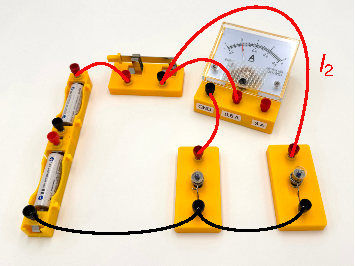
\includegraphics[width=4.6cm]{_images/ampere_parallel_2.pdf}
    \end{subfigure}
\quad
    \begin{subfigure}[b]{0.305\textwidth}
    \centering
    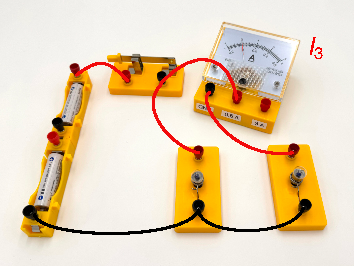
\includegraphics[width=4.6cm]{_images/ampere_parallel_3.pdf}
    \end{subfigure}
\end{figure}


% Raster für die Antworten
\begin{tikzpicture}
    \draw[step=4mm,gray,very thin] (0,0) grid (14.8,-14);

    \node  at (3.5,-3.5)
        {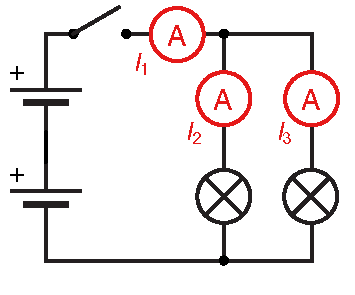
\includegraphics[width=6cm]{_images/ampere_parallel}};

        \draw (8,-1.85) node[anchor=north west,align=left,text width=13cm] {%
      		\marker%

            I$_{\text{1}}$ = \answer{0.44 A}  \\
            I$_{\text{2}}$ = \answer{0.22 A} \\
            I$_{\text{3}}$ = \answer{0.22 A}  \\

        };

        \draw (1,-6.6) node[anchor=north west,align=left,text width=13cm] {%
      		\marker%

            Fazit\\
            \answer{Die Stromstärke vor dem Knoten ist gleich der Summe der Stromstärken
            nach dem Knoten.}

        };
\end{tikzpicture}
